\documentclass[10pt, conference]{IEEEtran}
\usepackage{cite}
\usepackage{amsmath,amssymb,amsfonts}
\usepackage{algorithmic}
\usepackage{graphicx}
\usepackage{textcomp}
\usepackage{balance}
\usepackage{comment}
\usepackage[group-separator={,}]{siunitx}
\usepackage{grffile}
\usepackage{subcaption}
\usepackage{lipsum}
\usepackage{float}


\usepackage[T1]{fontenc}
\def\BibTeX{{\rm B\kern-.05em{\sc i\kern-.025em b}\kern-.08em
    T\kern-.1667em\lower.7ex\hbox{E}\kern-.125emX}}

%%%%%%%%%%%%%%%%% Macros %%%%%%%%%%%%%%%%%

\newcommand{\vectorScheme}{\textit{Vector Scheme}}
\newcommand{\valueScheme}{\textit{Value Scheme}}
\newcommand{\distanceScheme}{\textit{Distance Scheme}}
\newcommand{\distanceLemma}{\textit{Distance Lemma}}
\newcommand{\sketchScheme}{\textit{Sketched Change Scheme}}
\newcommand{\fullSync}{\textit{Full Sync}}
\newcommand{\naiveScheme}{\textit{Naive Scheme}}
\newcommand{\oracleScheme}{\textit{Oracle Scheme}}

%%%%%%%%%%%%%%%%% Document %%%%%%%%%%%%%%%%%
\begin{document}

%%%%%%%%%%%%%%%%% Title %%%%%%%%%%%%%%%%%
\title{Bandwidth Efficient Distributed Monitoring Schemes}
\author{
\begin{tabular}{c c c}
Yuval Alfassi & Dani Keren & Moshe Gabel \\
\textit{Computer Science Department} & \textit{Computer Science Department} & \textit{Computer Science Faculty} \\
\textit{University of Haifa} & \textit{University of Haifa} & \textit{Technion} \\
Haifa, Israel & Haifa, Israel & Haifa, Israel \\
yuvalalfassi@gmail.com & dkeren@cs.haifa.ac.il & mgabel@cs.technion.ac.il\\
\ & \ & \ 
\end{tabular} \\
\begin{tabular}{c c c}
Assaf Shuster & \ \ \ \ & Gal Yehuda \\
\textit{Computer Science Faculty} & \ \ \ \ & \textit{Computer Science Faculty} \\
\textit{Technion} & \ \ \ \ & \textit{Technion} \\
Haifa, Israel & \ \ \ \ & Haifa, Israel \\
assaf@cs.technion.ac.il & \ \ \ \ & gal2016@gmail.com \\
\ & \ \ \ \ & \ 
\end{tabular}
}
\maketitle

%%%%%%%%%%%%%%%%% Abstract %%%%%%%%%%%%%%%%%
\begin{small}
\textbf{
\textit{Abstract}--- Distributed monitoring is a problem that arises when trying to monitor properties of dynamic data which is spread distributively. Tracking the value of a function over dynamic data in a distributed setting is a challenging problem in numerous real-world modern applications. Several monitoring schemes were proposed as an approach to coping with this problem in order to reduce the amount of communication messages between servers, as well as the communication bandwidth. \\
Here, we propose several new distributed monitoring schemes using much less communication bandwidth. Existing schemes send high dimensional vectors from server to server while we propose some innovative methods for reducing the dimensionality of the transmitted data.\\
One scheme we propose is the \valueScheme \ which exploits some traits of convex functions, and another is the \distanceScheme \ which treats the function monitoring problem as a geometric monitoring problem, thereby utilizing geometric distances for distributed monitoring. \\
Moreover, we present a clever way to incorporate data-sketches into the schemes, which influence the bandwidth as well, allowing for some monitoring trade-offs to be made, depending on the sketch size.  }
\end{small}

%%%%%%%%%%%%%%%%% Introduction %%%%%%%%%%%%%%%%%
\section{Introduction}
Monitoring a function over large amount of dynamically changed data in a distributed fashion is a common computer-science challenge. Whether it's monitoring features of large distributed dynamic graphs [*] or multiple air pollution sensors [**], innovative approaches had to be developed in order to deal with the difficulties of both the data being dynamic and distributed. \\
The need of minimizing both the bandwidth and the processing power is expressed in [*]; a good example is internet of things objects which are operated on batteries, hence sending data via a communication channel is very costly, thus should be minimized. Furthermore, in the \textit{Big Data} era, when data is of very high dimensionality and changes rapidly, sending the whole data is not only impractical, but also extremely time consuming; for instance, air pollution sensors which distributively have to determine the air pollution level may benefit from an economical communication approach [***]. \\
Previous works were made on linear functions [*], where the linear properties make the distributed monitoring much easier; though in order to monitor non-linear functions a handful of difficulties arise. Works were done on distributively monitoring the entropy of distributed streams [*], monitoring the inner-product value of distributed dynamic vectors [**], and monitoring the number of triangles of dynamic graphs held in distributed servers [***]. \\
It should be noted that the classic approach to monitor distributed dynamic data is to send the data changes at a certain frequency  to a central server, called \textit{the coordinator}. This method may miss peaks of critical global data-changes, and also may be more expensive communication-wise -- not only data will be sent even when little changes are made, but the whole big dimensional data changes will be transmitted which might be extremely expensive. \\
The distributed monitoring problem is defined as follows:
\begin{enumerate}
\item There are $n$ servers and a coordinator. \\ $server_i$ maintains its dynamic \textit{local vector} $v_i$. \\ The \textit{global vector} is the average of the local vectors: $$v = \frac{1}{n}\sum\limits_{i=1}^n {v_i}$$
\item A function $f$ is monitored over the \textit{global vector} $v$ so it is $\varepsilon$-approximated with 100\% accuracy. \\ Let the estimation  be the value $\mu$ and ${f(v) \geq 0}$, than at all times: $$(1-\varepsilon )f(v) \leq \mu \leq (1+\varepsilon )f(v)$$
\end{enumerate}
The monitoring is done by bounding the function $f$ with a 'convex bound' function [*] -- a function $c$ which bounds the function from above (below) and used for the upper (lower) threshold monitoring.
Given a fucntion $f$ to monitor and a starting global vector $v_0$, it was proposed to approach the problem by finding a convex function $c$ which bounds the function $f$ i.e. for all $v$, ${f(v) \leq c(v)}$ and preferably ${f(v_0)=c(v_0)}$ [**]. \\
The function's approximation problem can be reduced to \textit{threshold monitoring problem} [*] where one monitors whether the function's value crosses a certain threshold. specifically, let $T$ be the threshold's value, than the general upper-bound monitoring objective is to determine whether:
\begin{equation}
\label{functionMonitoringConstraint}
f(v) \leq T
\end{equation}
and since ${f(v) \leq c(v)}$ for all $v$, we'd monitor whether:
\begin{equation}
\label{monitoringConstraint}
c(v) \leq T
\end{equation}
In turn, this threshold monitoring can be treated as a \textit{geometric monitoring problem} [***], where there's a \textit{valid zone} of vectors ${\{v \ | \ c(v) \leq T\}}$, which since $c$ is a convex function, every linear combination of vectors inside the \textit{safe zone} is also inside the \textit{safe zone}. 
\subsection{Contributions}
\begin{enumerate}
\item Introducing multiple innovative distributed monitoring schemes which avoid sending big dimensional data unless its crucially critical.
\item Proving the \distanceLemma , a lemma used as a basis of a distributed monitoring scheme we present. The \distanceLemma \ states that given a convex body and several points, if the sum of distances to the convex border from the points inside the convex body is greater than the sum of distances to the border from the points on the outside, than the average of the points is inside the convex body.
\item Incorporating data-sketches into distributed monitoring schemes without damaging the 0\% false-negative necessity of the distributed monitoring problem;e.g., we managed to prevent having the probabilistic nature of the sketches affect the distributed monitoring scheme having a false-negative result.
\item Conducting several experiments, laying out comparisons of multiple attributes of distributed monitoring schemes on real-world data, focusing on the bandwidth consumption.
\end{enumerate}

%%%%%%%%%%%%%%%%% Previous Work %%%%%%%%%%%%%%%%%
\section{Previous Work}
**** Consult with Dani on this part **** \\
(1) Linear Functions \\
(2) Covering Spheres \\
(3) Convex Decomposition

%%%%%%%%%%%%%%%%% Vector Scheme %%%%%%%%%%%%%%%%%
\section{Vector Scheme}
The \vectorScheme 's idea is to balance the server's data vectors whenever a local vector gets out of the function's convex bound. The \vectorScheme \ would try to balance the \textit{violated server} with other server's data vectors. It is done by incorporating \textit{slack vectors}, namely, $server_i$ would maintain a slack $\overrightarrow{s_i}$. It's important to note that the \vectorScheme \  makes sure that at all times the sum of the slacks is zero: ${\sum{\overrightarrow{s_i}} = 0}$.
In order to take into consideration these \textit{slacks}, a server raises a violation and initiates a communication channel with the coordinator if ${c(v_i+s_i)}$ exceeds the threshold; specifically, for an upper bound threshold, when ${c(v_i+s_i) > T}$. This ensures that whenever all the local constraint hold, the global constraint (\ref{monitoringConstraint}) holds. proof due to convexity of $c$, sum of slacks is zero and ${c(v_i+s_i) \leq T}$:
\begin{equation}
\label{vectorSchemeProof}
\begin{aligned}
 c(v)  \
	   &=  c\left(\frac{1}{n} \sum\limits_{i=0}^{n}{v_i}\right)  \
        =  \frac{1}{n} c\left(\sum\limits_{i=0}^{n}{(v_i + s_i)}\right) \\
      &\leq   \frac{1}{n} \sum\limits_{i=0}^{n}{c(v_i + s_i)}
       \leq   \frac{1}{n}(n \cdot T)
       = T
\end{aligned}
\end{equation}
When a violation occurs, i.e. ${c(v_i+s_i) > T}$ at a certain server, (\ref{vectorSchemeProof}) cannot longer be proven so a \textit{violation resolution protocol} has to occur.
\subsection{Violation Resolution}
In the \textit{violation resolution} phase, the slack vectors are balanced so ${c(v_i+s_i)}$ at the violated server would get inside the convex zone. When a server detects a local violation, it sends its local vector ${(v_i + s_i)}$ to the coordinator, which polls other servers for their local vectors as well. When the average of those vectors is inside the convex zone, i.e. ${c(E(v_i + s_i)) \leq T}$ the resolution is almost done, and no more servers have to be polled. Let ${(k-1)}$ be the number of polled servers, then the coordinator sends the average vector --- ${\frac{1}{k}\sum{(v_i + s_i)}}$ to the polled servers as well as the violated server, which update their slack to be ${s_j \leftarrow -v_j + \frac{1}{k}\sum_i{(v_i + s_i)}}$. Note that the sum of the slack vectors is still zero. \\
When all the servers are polled and the average vector still isn't inside the convex zone, a \textit{full sync} has to be done; Since the coordinator knows each server's ${(v_i + s_i)}$, the coordinator can calculate the global vector $v$, and hence $f(v)$. Then, the upper bound and lower bound are reset to ${(1 \pm \varepsilon )f(v)}$ and the monitoring continues with the coordinator notifying the servers of the new bounds and their local vector -- $v$ and their new slack -- the zero vector.
\subsection{Communication Bandwidth}
Considering the data vectors are of very high dimension, this scheme sends the whole vectors whenever even the slightest violation occurs. Therefore, even though the \vectorScheme \  is better than the naive monitoring scheme, its still wasteful in communication bandwidth.

%%%%%%%%%%%%%%%%% Value Scheme %%%%%%%%%%%%%%%%%
\section{Value Scheme}
The \valueScheme \ is a distributed monitoring scheme which reduces the bandwidth from sending a whole high dimensional vector to sending just one scalar.  Though, due to the dimensional reduction, we'd expect more false alarms to occur than at the \vectorScheme , and thus require more \textit{full syncs}. The scalar that will be passed will represent the \textit{value} of the convex bound function.\\
The \valueScheme \  maintains local scalar slack values; $server_i$ maintains the scalar $\lambda _i$. Also, at all times we'd enforce that the sum of the slacks is zero: ${\sum{\lambda _i} = 0}$. Here, the local server's constraint is whether ${c(v_i) + \lambda _i \leq T}$; hence, if all the local constraints are being held, the global constraint (\ref{monitoringConstraint}) will be held as well:
\begin{equation}
\label{valueSchemeProof}
\begin{aligned}
 c(v)  \
	    &=   c\left(\frac{1}{n} \sum\limits_{i=0}^{n}{v_i}\right)  \
       \leq   \frac{1}{n} \sum\limits_{i=0}^{n}c(v_i) \\
        &=    \frac{1}{n} \sum\limits_{i=0}^{n}{(c(v_i) + \lambda _i)}
       \leq   \frac{1}{n}(n \cdot T)
        = T
\end{aligned}
\end{equation}
When a violation occurs, i.e. ${c(v_i) + \lambda _i > T}$, proof (\ref{valueSchemeProof}) cannot longer hold, thus a violation resolution protocol has to be initiated.
\subsection{Violation Resolution}
The violation resolution protocol goes as follows: the violated server $server_i$ sends its local value ${c(v_i) + \lambda _i}$ which exceeds the threshold. The coordinator tries to 'balance' this scalar value by gradually polling other servers for their ${c(v_i) + \lambda _i}$ value. Let ${(k-1)}$ be the number of polled servers plus the violated server, then, when ${\frac{1}{k}\sum{(c(v_i) + \lambda _i)} \leq T}$ the violation will be resolved by sending ${\frac{1}{k}\sum{(c(v_i) + \lambda _i )}}$ to the polled servers and the violated server, which in turn, will set their local scalar slack to ${\lambda _j \leftarrow -c(v_j) + \frac{1}{k}\sum{(c(v_i) + \lambda _i)}}$. Its important to note that the sum of the slacks is zero after the resolution, and ${c(v_i) + \lambda _i \leq T}$ as well. \\
In case all the servers are being polled without being able to 'balance' the slack, a \textit{full sync} has to be done, which is very expensive regrading the communication bandwidth.
\subsection{Communication Bandwidth}
In the \valueScheme , the whole distributed monitoring is reduced to tracking one scalar value. The transmitted data is just one scalar instead of a whole high dimensional vector, as in \vectorScheme . Thus, we'd expect having much less communication bandwidth in this monitoring scheme.

%%%%%%%%%%%%%%%%% Distance Scheme %%%%%%%%%%%%%%%%%
\section{Distance Scheme}
The \distanceScheme \ is one more \textit{distributed monitoring scheme} that relies on passing a single scalar when communicating. This scheme, treats the distributed monitoring problem as a \textit{geometric monitoring problem}, where there's a geometric \textit{safe zone}, ${\{v \ | \ c(v) \leq T\}}$ where it's valid for local vectors to be at. The scalar that will be passed in the monitoring represents the \textit{distance} of the local vector at the server to the boundary of this convex bound.\\
This scheme is based on the \textit{Distance Lemma} which is proved below.
\subsection{The Distance Lemma}
The \distanceLemma \ states that the average of points is inside a convex body, if the sum of distances to the surface of the points inside the convex body is greater than the sum of distances to the boundary of the points which are outside of the convex body. This \textit{Distance Lemma} is the basis of the \distanceScheme . \\
The \distanceLemma : Let ${\{v_1 ... v_n\}}$ be vectors and let $C$ be a convex body. If the sum of the distances to the boundary of $C$ of the vectors inside $C$ is greater than the sum of the distances to the boundary of the vectors from outside, then the average vector ${\frac{1}{n}\sum {v_i}}$ is inside the convex set. \\
proof: \\
\begin{enumerate}
\item Let ${p_1 ,..., p_k}$ be the points inside the convex body $C$ and ${l_1 ,..., l_k}$ their distances to the boundary.
\item Let ${q_1 ,..., q_m}$ be the points outside the convex body $C$ and ${d_1 ,..., d_m}$ the distance vectors from the boundary to the points. Let ${c_1 ,..., c_m}$ be the points on the boundary which are the source of the distance vectors ${d_1 ,..., d_m}$ respectively.
\item Let ${d = \sum {d_i}}$ and ${l = \sum {l_i}}$
\item Assume $l \geq d$
\item It's needed to prove the average vector is inside the convex body, i.e., prove that ${\frac{1}{k+m}(\sum{p_i} + \sum{q_i}) \in C}$:
\end{enumerate}
\begin{equation}
\begin{aligned}
&( p_1+...+p_k) + (q_1+...+q_m) = \\
&( p_1+...+p_k) + (c_1+d_1) + ... + (c_m + d_m) = \\
&( p_1+...+p_k) + d + (c_1 + ... + c_m) = \\
&\left( p_1 + \frac{l_1 d}{l}\right) + ... + \left(p_k + \frac{l_k d}{l}\right) + (c_1 + ... + c_m)
\end{aligned}
\end{equation}
\begin{enumerate}
\item[\ \ \ ] ${c_i \in C}$ by definition -- $c_i$ is on the boundary of $C$. Also, ${p_i + \frac{l_i d}{l} \in C}$ because ${l \geq d}$ and $l_i$ is the distance of $p_i$ to the boundary. \\
Since an average of points inside a convex body is also inside the convex body, ${\frac{1}{k+m}(\sum{p_i} + \sum{q_i}) \in C \ \blacksquare} $ 
\end{enumerate}
\subsection{Distributed Monitoring}
The \distanceScheme \ is based on the distance value of the local vectors to the convex geometric boundary. The \distanceScheme \ literally monitors distributively whether the sum of the distances from inside to the boundary is greater than the sum of the distances to the boundary from the outside. For convenience, denote the distance to the boundary from inside the convex body as negative, and the distance from outside as positive, therefore, the \distanceScheme \ monitors whether the sum of the distances is negative. \\
Like the \valueScheme , the \distanceScheme \ maintains slack scalars that would help 'balance' the distances from the boundary between servers as data changes. Let $server_i$ maintain the scalar $\lambda _i$. As in \valueScheme , at all times the sum of the slacks is zero: ${\sum {\lambda _i} = 0}$. \\
Denote $d_i$ the distance of $server_i$'s vector to the boundary, then the local server's monitoring constraint is whether ${d_i + \lambda_i \leq 0}$. Therefore, if all the local constraints hold, the global vector's distance is negative and by the \textit{Distance Lemma}, the global constraint (\ref{monitoringConstraint}) holds:
\begin{equation}
\sum{d_i} = \sum{(d_i + \lambda _i)} \leq n \cdot 0 = 0
\end{equation}
The sum of the distances is negative, thus the average vector is inside the convex set. \\
Whenever ${d_i + \lambda _i > 0}$ at a certain server, a violation occurs and a  \textit{violation resolution protocol} has to occur. 
\subsection{Violation Resolution}
When the local vector at a server changes so ${d_i + \lambda _i > 0}$, a violation occurs. In order to resolve the violation, the $\lambda _i$ slacks has to be balanced so ${d_i + \lambda _i \leq 0}$ at the violated server as well as other servers where some slack would be 'borrowed'. \\
Firstly, in order to resolve the violation, the violated server sends its ${d_i + \lambda _i}$ value to the coordinator; afterwards, the coordinator gradually polls others servers for their ${d_i + \lambda _i}$ value. Let $(k-1)$ be the number of polled servers, than when ${\frac{1}{k}\sum(d_i + \lambda _i) \leq 0}$ the violation can be resolved, and the coordinator sends the single value ${\frac{1}{k}\sum(d_i + \lambda _i)}$ to the polled servers and the violated server. Then, the slacks are updated so ${\lambda _j 
\leftarrow -d_j + \frac{1}{k}\sum(d_i + \lambda _i)}$. Note that the sum of slacks is still zero after the update, and at each server the local constraint holds, ${d_i + \lambda _i \leq 0}$.
\subsection{Communication Bandwidth}
The monitoring is done solely by the value of the distance. A scalar value is transmitted between the coordinator and the servers, thus we'd expect much less communication bandwidth than the \vectorScheme .

%%%%%%%%%%%%%%%%% Data Resolution %%%%%%%%%%%%%%%%%
\section{Sketched Change Scheme}
The \sketchScheme \ is an integration of the \vectorScheme \ and either the \valueScheme \ or the \distanceScheme . \\
This scheme behaves like the \valueScheme \ or the \distanceScheme \ up until a violation which the one dimensional scheme cannot resolve and a \fullSync \ has to be made. Instead of the \fullSync \ , the coordinator polls the servers for a \textit{sketch} of their change vector of the data. the average of the sketches is combined and sent to the servers, which benefit some data from it. For the sketch function, multiple functions can be used, such as sending the most dominant element of the vector, the most dominant DCT parameters of the vector and the most dominant PCA parameters. \\
The better the sketch represents the change vector, more beneficial information the servers will have which will help overcome the violation occurred. \\
Simply, the \sketchScheme \ allows more soft and gradual \fullSync \ to be done. If this partial \fullSync \ still won't allow the one-dimensional distributed monitoring scheme to be continued, the dimension of the sketch will be raised so the \fullSync \ would be more representative of the global vector. \\
\subsection{Distributed Monitoring}
The algorithm of the \sketchScheme \ is as follows:
\begin{enumerate}
\item Choose a one-dimensional distributed monitoring scheme, note it $d$.
\item Distributively monitor the global monitored functional according to $d$.
\item when a \fullSync \ has to be invoked, send a sketch of the 
\end{enumerate}
.....

\begin{figure*}[t]
\begin{minipage}[b]{0.5\linewidth}
\centering
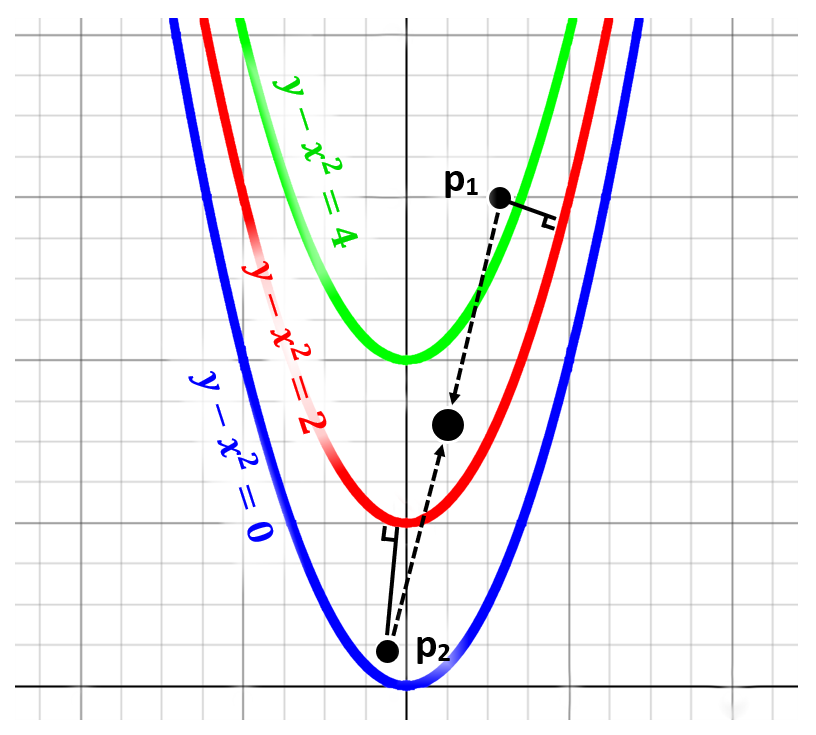
\includegraphics[width=\textwidth]{Pics/distanceSchemeFails.PNG}
\caption{\valueScheme \ beats \distanceScheme}
\label{fig:valueBeatsDistanceFigure}
\end{minipage}
\begin{minipage}[b]{0.5\linewidth}
\centering
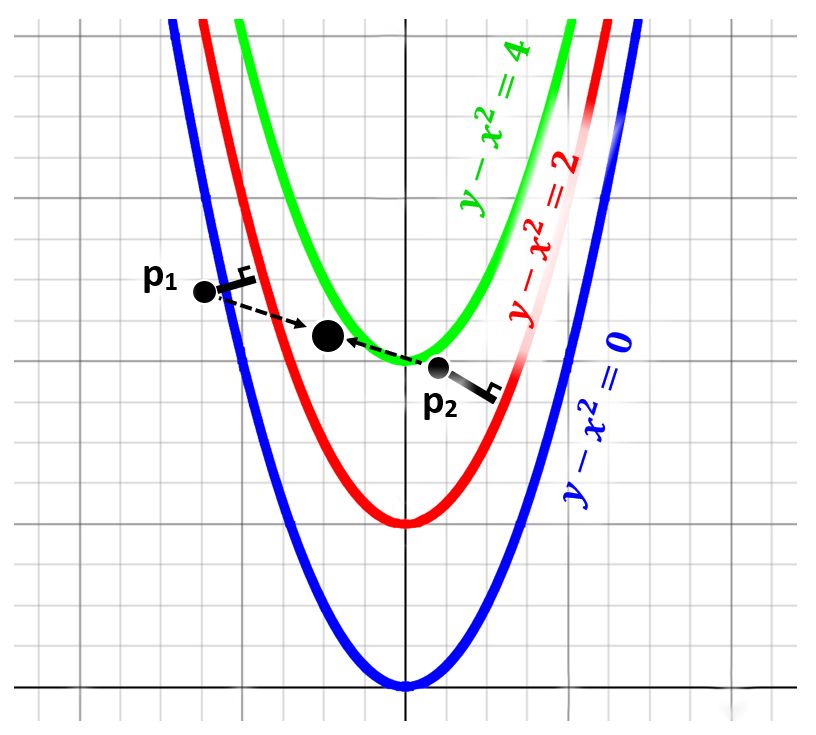
\includegraphics[width=\textwidth]{Pics/valueSchemeFails.PNG}
\caption{\distanceScheme \ beats \valueScheme}
\label{fig:distanceBeatsValueFigure}
\end{minipage}
\medskip

\small
When monitoring the convex condition ${f(x) = y - x^2  \geq 2}$, there are cases of false negative violations which occur only in one distributed monitoring scheme and not the other. The global average vector remains inside the convex bound ${f(x) \geq 2}$ while a false alarm can be raised. In Fig. (\ref{fig:valueBeatsDistanceFigure}) the distance to the boundary $f(x) = 2$ from the outside point $p_2$ is greater than the distance from the point inside - $p_1$, though ${\frac{1}{2}(f(p_1)+f(p_2))\geq 2}$ , so the \valueScheme \ won't raise a violation, while the \distanceScheme \ will raise a violation which is a false alarm. \\
In Fig. (\ref{fig:distanceBeatsValueFigure}) the distance to the boundary $f(x) = 2$ of the point inside $p_2$ is greater of the distance of the point outside, $p_1$, however, ${\frac{1}{2}(f(p_1)+f(p_2))\leq 2}$, so the \valueScheme \ will raise a false-negative violation, while the \distanceScheme \ correctly won't raise a violation.
\end{figure*}

\subsection{Violation Resolution}
The violation resolution of the \sketchScheme \ is invoked when the one-dimensional monitoring scheme fails. 
\begin{enumerate}
\item Let $n$ be the number of servers. Let $r$ be their reference vectors and $ch_1 ... ch_n$ be their data-change vectors.
\item Let $d$ be the chosen dimension of the violation resolution.
\item Let $sk_d$ be a sketch function of dimension $d$. Let $sk_d (ch_i)$ be the sketch of the change vector of the i-th server, and $\varepsilon _d$ be the 'error' of the sketch function so ${ch_i = sk_d(ch_i) + \varepsilon _i}$ for all $server_i$.
\item Each server sends its $sk_d(ch_i)$ to the coordinator.
\item The coordinator calculates the average of the sent vectors ${\overline{sk_d} = \frac{1}{n}\sum sk_d(ch_i)}$ and transmits it to the servers.
\item Each server $server_j$ will update its reference vector to be ${r \leftarrow r + \overline{sk_d}}$ (the reference vector is the same at all servers). The change vectors are updated as well: ${ch_j \leftarrow \varepsilon _i}$.
\item Set the value/distance scalar slacks of the vectors to zero and try continuing the one-dimensional distributed scheme.
\item if the one-dimensional scheme immediately tries to invoke a \fullSync \ again, raise the sketch dimension to $2\cdot d$ up to $\frac{n}{2}$.
\item if a violation reoccurs when ${d \geq \frac{n}{2}}$ invoke a \fullSync .
\end{enumerate} 
It's important to note that at all times before and after the violation, the global vector remains the same: ${v = \frac{1}{n}\sum v_i}$. Moreover, the 'error' of the sketch function is taken into account so there's no probabilistic nature to this scheme. As the sketch function represents the change better, the local vector of the server is estimates better the global vector and is closer to it.
\subsection{Communication Bandwidth}

%%%%%%%%%%%%%%%%% Value Scheme vs. Distance Scheme %%%%%%%%%%%%%%%%%
\section{Value Scheme vs. Distance Scheme}
Both \valueScheme \ and \distanceScheme \ are distributed monitoring schemes which are reduced to tracking just one scalar value. In the \distanceScheme \ its the sum of the distances to the convex bound's geometric boundary, and in the \valueScheme \ its the average of the convex function's value. \\
A good question that arises is which monitoring scheme is better? which one uses less communication bandwidth? Is there a connection between the schemes? \\
In [*] its proposed theres a connection between the distance to a function and the value of the function. moreover, when the distance is small, there's a linear correlation between the function's value and the distance. \\
Nonetheless, since we are dealing with convex functions, the value grows faster than the function's value. A good example is the function ${f(v) = (\sum v_i)^{100}}$ which  when monitoring ${f(v) \leq 1}$, the function's value changes rapidly outside the boundary, whereas the distance changes regularly.
This behavor is showed in the experiment done in section [**] on the function ${f(v) = ||v||^2}$. \\
Even though in convex functions the distance grows faster than its value, it doesn't necessarily imply that the distance scheme is better. for example, monitoring the convex condition $y-x^2 \geq 2$, the results aren't conclusive. As shown in (....) (add paintings)
(.....)
Another important factor is that the \valueScheme \ is computationally mathematically whole, while the \distanceScheme \ may require some approximations. The problem of finding the distance to the convex bound from outside is mathematically closed using convex optimization techniques. On the other hand, finding the distance from inside to the convex body isn't always solvable [**], so the \distanceScheme \ isn't applicable in all the possible functions that require distributed monitoring.


%%%%%%%%%%%%%%%%% Experimental Results %%%%%%%%%%%%%%%%%
\section{Experimental Results}
In order to assess the productivity of the distributed monitoring schemes proposed, we tested the communication bandwidth of the data sent between the servers and the coordinator both on real-world diverse data and synthetic scheme-oriented data. \\
As for the distributed dynamic monitored data, we used a bag-of-words [*] vector of high dimension constructed of occurrences of tokens in a moving sliding window in the servers. The servers data is diverse: one is created out of blogs from \textit{bloggers.com} while other is fed of tweets posted online etc. 
\subsection{Oracle Scheme and Naive Scheme}
One of the needs of comparing between the monitoring schemes and assessing whether the monitoring schemes proposed really are economical bandwidth-wise is offering a lower-bound and an upper bound for distributed monitoring schemes. \\
The obvious communication-bandwidth upper bound is the \naiveScheme \ which simply sends each data change at a server to the coordinator. This method obviously isn't very bandwidth efficient, though its a good upper bound.
For the lower bound of the communication bandwidth, we propose the \oracleScheme \ which is like an oracle which knows it all. Simply, whenever a true violation occurs, i.e. ${f(v') > (1
+\varepsilon)f(v)}$ or ${f(v') < (1-\varepsilon)f(v)}$ (for simplicity, ${f(v) \geq 0}$), a \fullSync is invoked. Of course this scheme isn't realistic, since a server knows nothing about its neighbours, so the global vector isn't known. In other words, data is transmitted only when its truly needed to be passed -- a \fullSync \ must be done.
\subsection{Norm $L_2$ Squared}
The norm $L_2$ is used in multiple scenarios, as in [*] and [**]. Monitoring this function distributively isn't Obvious even though the function is convex. \\
Here, we monitored the $L_2$ norm squared, namely $f(v) = ||v||^2$. One of the reasons is to confirm that this function is better bandwidth-wise using the \distanceScheme \ in contrast of the \valueScheme . \\
Finding the convex bound of the function isn't difficult since it's convex. the upper bound is the function itself, and the lower bound's convex function is the tangent plane to the function at the closest point to the global vector with norm squarred as the lower bound's threshold. \\
To check the difference between the \valueScheme \ and \distanceScheme \ we constructed one hundred servers with a vector in dimension $\num[group-separator={,}]{10000}$. The servers dynamically change. The changes were of small steps in all the $\num[group-separator={,}]{10000}$ dimensions. \\
The bandwidth results over time are presented in figure [***]. For this experiment we monitored the function by bounding it ${(\pm 10)}$ instead of a multiplicative ${(1 \pm \varepsilon)f(v_0)}$.
\begin{figure}[b]
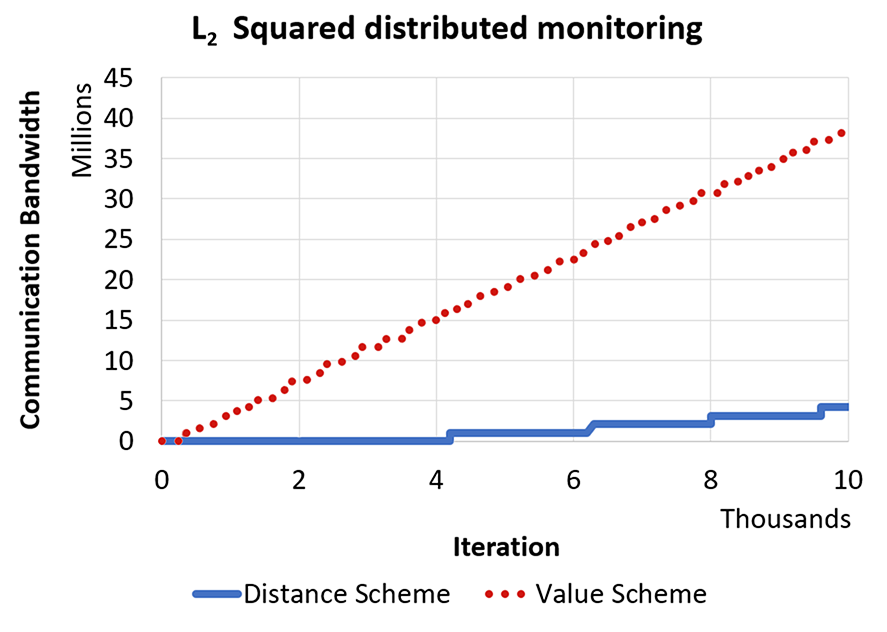
\includegraphics[width=\linewidth]{Pics/Sphere.PNG}
\label{SphereMonitoring}
\caption{\distanceScheme \ uses less communication bandwidth than \valueScheme \ when monitoring norm $L_2$ squared function}
\end{figure} 
\subsection{Inner Product}
\subsection{Entropy}

%%%%%%%%%%%%%%%%% Conclusions %%%%%%%%%%%%%%%%%
\section{Conclusions}

%%%%%%%%%%%%%%%%% References %%%%%%%%%%%%%%%%%
\begin{thebibliography}{00}
\bibitem{b1} G. Eason, B. Noble, and I. N. Sneddon, ``On certain integrals of Lipschitz-Hankel type involving products of Bessel functions,'' Phil. Trans. Roy. Soc. London, vol. A247, pp. 529--551, April 1955.
\bibitem{b1} G. Eason, B. Noble, and I. N. Sneddon, ``On certain integrals of Lipschitz-Hankel type involving products of Bessel functions,'' Phil. Trans. Roy. Soc. London, vol. A247, pp. 529--551, April 1955.
\bibitem{b1} G. Eason, B. Noble, and I. N. Sneddon, ``On certain integrals of Lipschitz-Hankel type involving products of Bessel functions,'' Phil. Trans. Roy. Soc. London, vol. A247, pp. 529--551, April 1955.
\bibitem{b1} G. Eason, B. Noble, and I. N. Sneddon, ``On certain integrals of Lipschitz-Hankel type involving products of Bessel functions,'' Phil. Trans. Roy. Soc. London, vol. A247, pp. 529--551, April 1955.
\bibitem{b1} G. Eason, B. Noble, and I. N. Sneddon, ``On certain integrals of Lipschitz-Hankel type involving products of Bessel functions,'' Phil. Trans. Roy. Soc. London, vol. A247, pp. 529--551, April 1955.
\bibitem{b1} G. Eason, B. Noble, and I. N. Sneddon, ``On certain integrals of Lipschitz-Hankel type involving products of Bessel functions,'' Phil. Trans. Roy. Soc. London, vol. A247, pp. 529--551, April 1955.
\bibitem{b1} G. Eason, B. Noble, and I. N. Sneddon, ``On certain integrals of Lipschitz-Hankel type involving products of Bessel functions,'' Phil. Trans. Roy. Soc. London, vol. A247, pp. 529--551, April 1955.
\bibitem{b1} G. Eason, B. Noble, and I. N. Sneddon, ``On certain integrals of Lipschitz-Hankel type involving products of Bessel functions,'' Phil. Trans. Roy. Soc. London, vol. A247, pp. 529--551, April 1955.
\bibitem{b1} G. Eason, B. Noble, and I. N. Sneddon, ``On certain integrals of Lipschitz-Hankel type involving products of Bessel functions,'' Phil. Trans. Roy. Soc. London, vol. A247, pp. 529--551, April 1955.
\bibitem{b1} G. Eason, B. Noble, and I. N. Sneddon, ``On certain integrals of Lipschitz-Hankel type involving products of Bessel functions,'' Phil. Trans. Roy. Soc. London, vol. A247, pp. 529--551, April 1955.
\bibitem{b1} G. Eason, B. Noble, and I. N. Sneddon, ``On certain integrals of Lipschitz-Hankel type involving products of Bessel functions,'' Phil. Trans. Roy. Soc. London, vol. A247, pp. 529--551, April 1955.
\bibitem{b1} G. Eason, B. Noble, and I. N. Sneddon, ``On certain integrals of Lipschitz-Hankel type involving products of Bessel functions,'' Phil. Trans. Roy. Soc. London, vol. A247, pp. 529--551, April 1955.
\bibitem{b1} G. Eason, B. Noble, and I. N. Sneddon, ``On certain integrals of Lipschitz-Hankel type involving products of Bessel functions,'' Phil. Trans. Roy. Soc. London, vol. A247, pp. 529--551, April 1955.
\bibitem{b1} G. Eason, B. Noble, and I. N. Sneddon, ``On certain integrals of Lipschitz-Hankel type involving products of Bessel functions,'' Phil. Trans. Roy. Soc. London, vol. A247, pp. 529--551, April 1955.
\end{thebibliography}

%%%%%%%%%%%%%%%%% End Document %%%%%%%%%%%%%%%%%
\end{document}
